\documentclass[11pt,english,a4paper] {report}
\usepackage[latin1]{inputenc}
\usepackage[T1]{fontenc}
\usepackage{babel,graphicx,varioref}
\usepackage{palatino}
\usepackage{relsize}
\usepackage{varioref}
\usepackage{pdfpages}
\usepackage{fancyvrb}
\usepackage{fancyhdr}
\usepackage{sectsty}
\usepackage{times}
\usepackage{hyperref}
\usepackage{amsmath}
\usepackage{geometry}

%For code listings
\usepackage{color}
\usepackage{xcolor}
\usepackage{listings}
\usepackage{courier}
\usepackage{pdfpages}
\usepackage{varioref}

\usepackage{dirtree}
\usepackage{fancyref}
\usepackage{float}

\definecolor{codegreen}{rgb}{0,0.6,0}
\definecolor{codegray}{rgb}{0.5,0.5,0.5}
\definecolor{codepurple}{rgb}{0.58,0,0.82}
\definecolor{backcolour}{rgb}{0.95,0.95,0.92}
\definecolor{keywordcolor}{RGB}{133,0,3}
\definecolor{commentcolor}{RGB}{135,136,117}
\definecolor{numbercolor}{RGB}{38,38,38}
\definecolor{stringcolor}{RGB}{211,0,53}

%\renewcommand*\rmdefault{Consolas, 'Liberation Mono', Menlo, Courier, monospace}

\def\ff{Consolas, 'Liberation Mono', Menlo, Courier, monospace}

\lstset{
    basicstyle=\scriptsize,%\fontfamily{\ff},
    numbers=left,               % Ort der Zeilennummern
    numberstyle=\scriptsize,%\tiny,          % Stil der Zeilennummern
    %stepnumber=2,               % Abstand zwischen den Zeilennummern
    numbersep=5pt,              % Abstand der Nummern zum Text
    tabsize=2,                  % Groesse von Tabs
    extendedchars=true,         %
    breaklines=true,            % Zeilen werden Umgebrochen
    %keywordstyle=\color{red},
    frame=b,         
    keywordstyle=[1]\textbf,    % Stil der Keywords
    keywordstyle=[2]\textbf,    %
    keywordstyle=[3]\textbf,    %
    %keywordstyle=[4]\textbf,   \sqrt{\sqrt{}} %
    %stringstyle=\color{white}\ttfamily, % Farbe der String
    showspaces=false,           % Leerzeichen anzeigen ?
    showtabs=false,             % Tabs anzeigen ?
    xleftmargin=17pt,
    framexleftmargin=17pt,
    framexrightmargin=5pt,
    framexbottommargin=4pt,
    %backgroundcolor=\color{lightgray},
    showstringspaces=false,%false      % Leerzeichen in Strings anzeigen ?        
    breakatwhitespace=false,
    keepspaces=true,
    commentstyle=\color{commentcolor},%\fontfamily{\ff},%codegreen},
    keywordstyle=\color{keywordcolor}\fontfamily{\ff}, %magenta},
    numberstyle=\tiny\color{numbercolor}\fontfamily{\ff}, %codegray
    stringstyle=\color{stringcolor}\fontfamily{\ff},%codepurple
    columns=fullflexible
 }
 \lstloadlanguages{
        Python,
        Bash
 }
    %\DeclareCaptionFont{blue}{\color{blue}} 

  %\captionsetup[lstlisting]{singlelinecheck=false, labelfont={blue}, textfont={blue}}
  %\usepackage{caption}
%\DeclareCaptionFont{white}{\color{white}}
%\DeclareCaptionFormat{listing}{\colorbox[cmyk]{0.43, 0.35, 0.35,0.01}{\parbox{\textwidth}{\hspace{15pt}#1#2#3}}}
%\captionsetup[lstlisting]{format=listing,labelfont=white,textfont=white, singlelinecheck=false, margin=0pt, font={bf,footnotesize}}
\usepackage{caption}
\DeclareCaptionFont{white}{\color{white}}
\DeclareCaptionFormat{listing}{\colorbox{gray}{\parbox{\textwidth}{#1#2#3}}}
\captionsetup[lstlisting]{format=listing,labelfont=white,textfont=white}
% done code

%\usepackage[colorlinks=true,pdfstartview=FitH, linkcolor=blue, 
            %citecolor=blue, urlcolor=blue,bookmarksopen=true]{hyperref}
\def\course{MS016A}
\def\reportname{Lab Report}
\def\name{Lars Haugan}
\author{Lars Haugan - s171201}
\def\studentnr{s171201}
\def\line{NSA}
\def\school{University of Oslo \\ Oslo and Akershus Univeristy College of Applied Sciences}
\def\semester{Autumn 2014}

\hypersetup
{
        pdftitle={\reportname},
        pdfauthor={\name},
        pdfsubject={\reportname},
        colorlinks=true,
        linkcolor=blue,
        citecolor=black,
        urlcolor=blue,
        pdfstartview=FitH,
        bookmarksopen=true
}

\usepackage{apacite}
\bibliographystyle{apacite}

\parindent=0in
\fvset{frame=single,framesep=3mm,fontfamily=helvetica,fontsize=\scriptsize}
\setlength{\parskip}{1em}

\renewcommand\ttfamily{\small\bf\fontfamily{helvetica}}
\newcommand{\HRule}{\rule{\linewidth}{0.2mm}}

\begin{document}
\begin{titlepage}
    \begin{center}

        \large \line\\
        \large \school\\ \semester\\[0.4cm]
        \HRule\\[1.5cm]
        \name, \studentnr
        \ \\[6.0cm]
        \LARGE\textbf{\course\ - \reportname}

    \end{center}
\end{titlepage}


%\title{  \course\ \reportname } %\\ \name \ - \studentnr }

\allsectionsfont{\sffamily}

\tableofcontents

\chapter{Dynamic cloud-based scaling web services}
\textbf{Keywords: Virtualization, Cloud computing, performance, scripting}

\subsection*{Abstract}

This report takes a look at the implementation of a dynamic setup in cloud-based
web-services that scale with the load. With the load balancer HAProxy and
implemented through OpenStack APIs.

\section{Introduction}

\subsubsection{Problem statement}

The given problem statement in this project was as follows:

\emph{Build a cloud-based web service which is able to adjust the number of
webservers based on the incoming rate of user requests.}

\section{Background}
Cloud computing is becoming more and more popular, and is being implemented
in many parts of the industry \cite{OpenStack:Users}. You can rent resources 
from large providers like Amazon which provides a public cloud infrastructure 
or by building your own cloud infrastructure. This can be done with open source 
tools like OpenStack. There is also a third alternative that is the hybrid cloud,
which enables easy transaction from using both a private cloud and public clouds.\\

Having these cloud infrastructures, make it possible to have services
that scale over multiple locations, and to utilize the resources that are
available. When having spanning clouds we can use this to our advantage 
and create solutions to create more sturdy solutions, that will scale web
services in a more cost efficient way.\\

Web services with many consumers or with a high demand for calculation power
will need to be able to use multiple servers to provide service to the clients.
The number of servers needed is proportionate to the number of visitors and
calculations needed to provide the service. If there is not enough servers to
handle the load, there will a result in long response times or even loss of
service.\\

To handle this we need a way of scaling the number of servers in a way that
will give the expected result for the consumers, but at the same time use the
bare minimum amount needed in able to save money.\\

This will make the basis for this chapter where we will look into a solution to
scale a web service over multiple servers in an OpenStack environment.

\subsection{Cloud solution with OpenStack}
OpenStack is a free open source cloud software, that can be used to provide
infrastructure as a service (IaaS). 
OpenStack proclaims to be one of the fastest growing open source communities in
the world, backed by some of the biggest names in the industry like
RedHat and HP \cite{OpenStack:2014}. It is built up of multiple services
where each is responsible to handle a part of the operation in the cloud. Most
notably of these are nova, which handles the instances it selves and the
communication with the vitalization hypervisor. There are a total of 13
services which handles everything from identities, storage, networking,
orchestration and much more.\\

OpenStack is a viable cloud solution due to the large scale implementation, and
the large community supporting further development. One of the features provided 
and result of the open source software are the APIs that are available. 
\textit{Python-novaclient} implementation that provides almost full integration
with nova. Other implementations for the other OpenStack services are also
available. Since OpenStack are implemented in Python, there has been more work
on these API implementations, than what you might expect from a open source
project. According to \cite{OpenStack:api_comparison} the nova API is
compatible with the implementation from Amazon (AWS). This means that it is
possible to use \textit{python-novaclient} also with AWS. This is powerful when
developing tools that are supposed to work with clouds.

\subsection{HAProxy for load balancing}
HAProxy (High Availability proxy) is a free, very fast and reliable solution offering
high availability, load balancing, and proxying for TCP and HTTP-based applications
\cite{haproxy:2014}. It is used by large sites like Reddit, Stack Overflow and
Twitter \cite{haproxy:they_use_it}. Some of the features it provides in the
latest version is native SSL/TLS termination, which is lacking from most other
freely available load balancers, full HTTP keep-alive, IPv6 support, health
checks and much more \cite{haproxy:2014}. There are other free load balancers
that can be used, such as apache with mod, nginx, pound and varnish. Varnish is
mostly used only for caching and does not support SSL/TLS termination. HAProxy
appears to be a de facto standard when it comes to open source load
balancers.\\

These solutions creates a background for the solution to be created that can
make a service scale in a cloud environment. All this so we can save money, and
serve solutions that will prevail with large amounts of requests.
It is also worth noting that it will not only save the provider money, but
ultimately lower energy usage that could lower the environmental impact of a
service.


\section{Approach}
This study will focus on creating a application that enables scaling of a web 
service in a cloud environment. It will explore the possibility of web scaling
by implementing the posibilities of OpenStack and HAProxy in a Python
application. 
This will make it possible to make an application that is tightly integrated
with both OpenStack and HAProxy and make good use of the tight integration.

\subsection{Setup}

\subsection{OpenStack integration}
OpenStack provides excellent possibilities for integration when programming in
Python. With the use of \textit{python-novaclient} it is possible to do almost
anything you can do with nova through either the CLI or OpenStack Horizon.

It is to be expected that the integration can provide all the needed
functionality of handling the instances. This means that it is possible to
handle the creation of new instances and provide the needed information so that
OpenStack handles the installation of the needed software on the new servers.
This can be done through the usage of cloud-data which is served with a
metadata service provided by OpenStack.

With this the application can scale up completely new instances which is
configured for the service within a short amount of time. When the instances
are no longer needed, the integration can shutdown or delete the instance
altogether.

\subsection{HAProxy integration}

\subsection{Needed data}
% Rate of incomming requests.

% How to scale based on the data

\subsection{Expected data}
% Output of the script

\subsection{How to test}

To be able to scale the web service based on the incomming count of requests,
there are multiple aspects that needs to be implemented. These include the
ability to create/start/stop/destroy instances (read: Virtual machines) and
monitor the number of incomming requests.


* Describe the design of the project
* How the data should look
* How to analyze the data

% Is the type of study explained?
% Are all the experiments explained?
% Are the assumptions explained?
% Are there limitations to the approach which you are aware of (NOT hindsight)?
% Is there an explained connection between the data you want to gather and the
% problem you investigate?

\subsection{Creating a webscaler}

\subsection{Data gathering and testing}

 %What is the claim
 %What to do
 %How do i test
 %Output
 %Optional approaches
 %Calcualtion differences
 %reqs
 %reactive \/ proactive

\section{Result}
 %What happened

\section{Analysis}
 %Look at the data
\begin{figure}[htp]
%\centering
%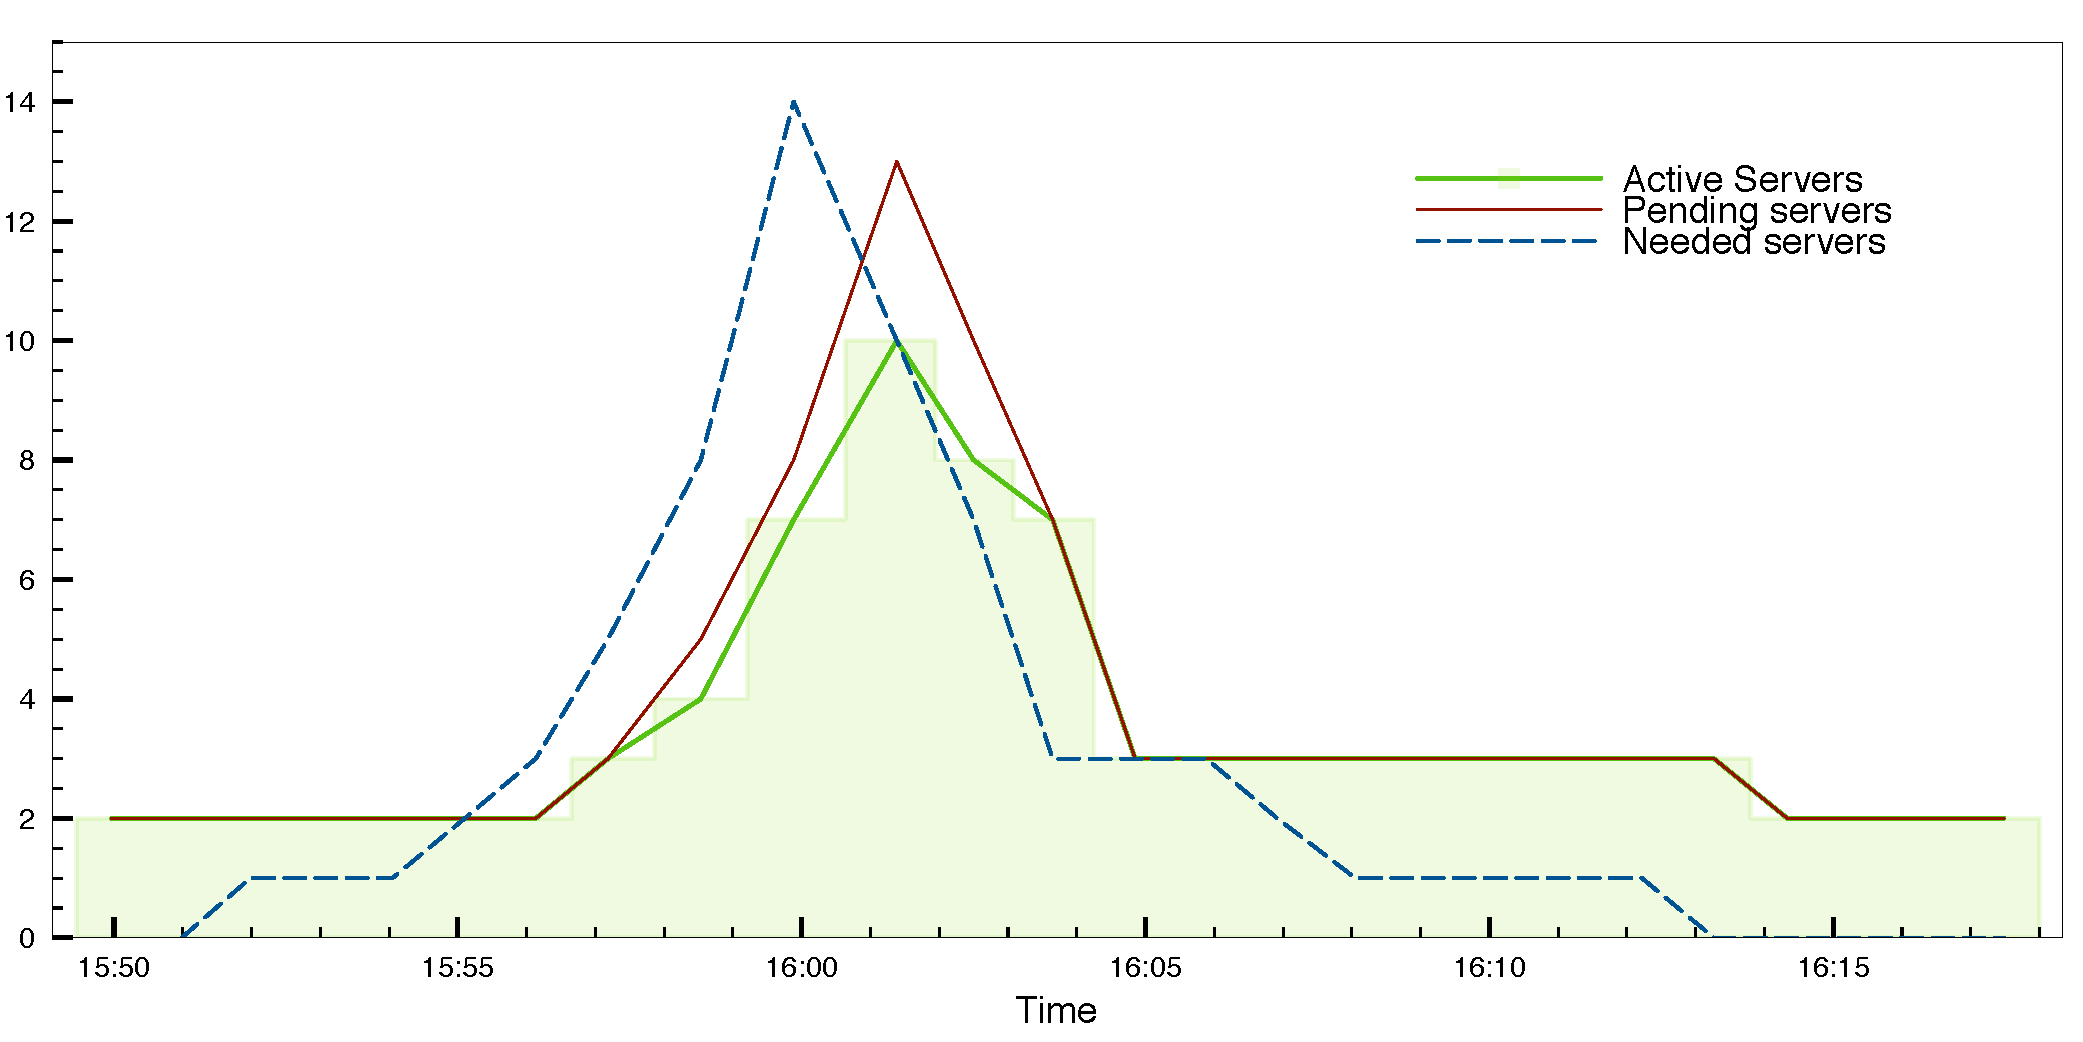
\includegraphics[scale=0.6]{chapter1/server_scaling}
\centering
\makebox[\textwidth][c]{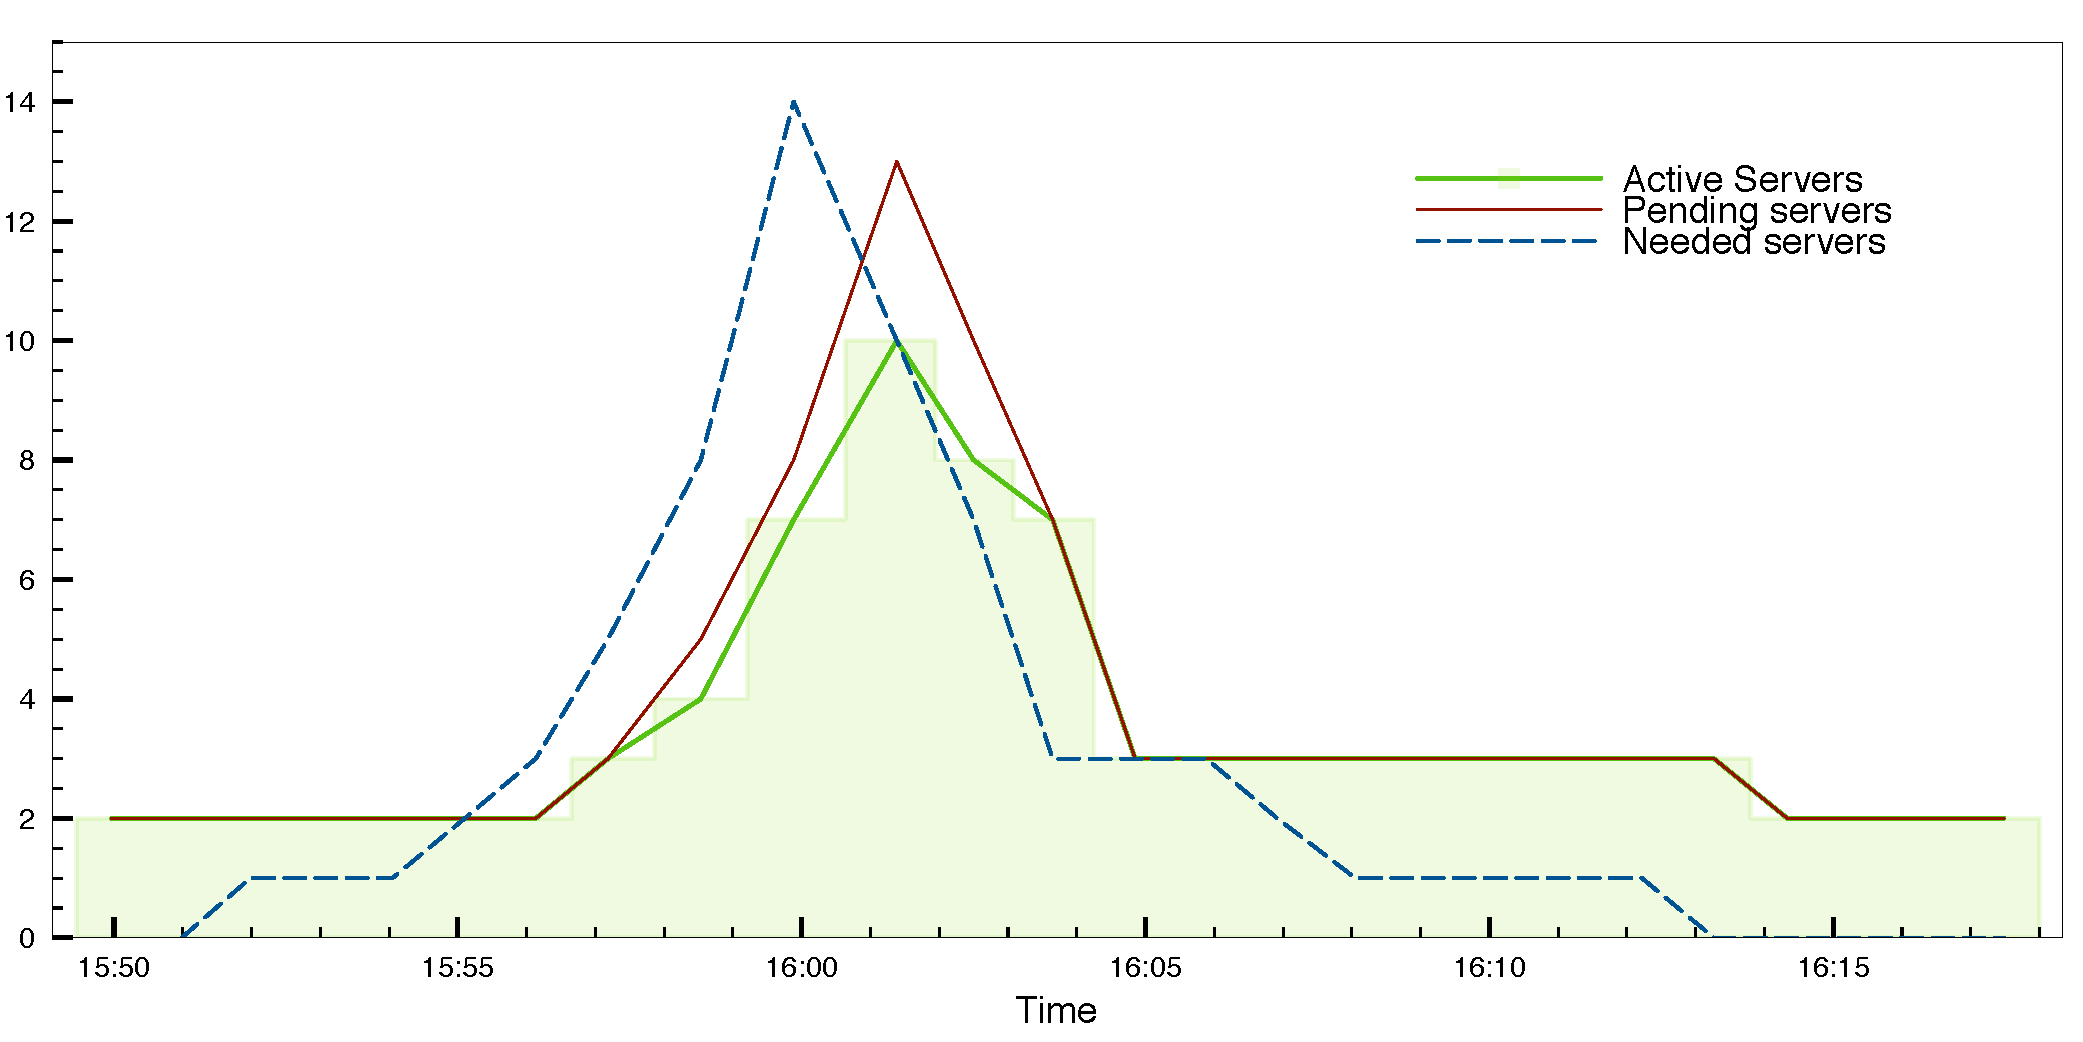
\includegraphics[width=1.2\textwidth]{chapter1/server_scaling}}
\caption{\label{fig:server_scaling}Scaling of servers}
\end{figure}

\section{Discussion and conclusion}
% Why did i not use MLN
\subsection{Improvements}

\subsection{Conclusion}



requests per seconds fornuftig kan vi forvente at en server toler akkurat
det vi har satt i forhold til at det er forskjellige urler


\chapter{Comparing HAProxy and Pound load balancers}
\textbf{Keywords: Webservers, Performance, Analysis}

\subsection*{Abstract}

\section{Introduction}

\subsubsection{Problem statement}

The given problem statement in this project was as follows:

\emph{Setup and evaluate and compare the perlbal and pound load balancers for a
web- service with regard to:
\begin{itemize}
    \item Configureability
    \item Performance
    \item Scalability
\end{itemize}}

\section{Background}
Load balancers are important to most of the high end websites that are
available. Ensuring high availability and great scalability. They can be a part
of even the smallest sites that are prone to fail, but that need high uptime,
or to balance the load over multiple webservers, or database servers.

% Talk about httperf

% Talk about HAProxy

% Talk about Pound

\section{Approach}
% How thing is supposed to be set up
% Hypothesis

% assumption: set of assumption for the different cases
% how the setup is
% The different cases:
    % httperf with increasing rate of requests and/or connections
        % naturally that there are multiple requests per connection

\section{Result}
%What happened
% Subsection: Configurability
%   Syntax? Functions, documentation, community and continuous support (new
%   versions?) This is relevant, but not directly to how it works. Evaluate
%   this!
%


% the data are presented as described in the approach section
% how are the tests run
% sample output of scripts and/or httperf
% present the data for the spesifik sets
    % how to find the data and how they were analyzed


% ssl signing: openssl req -x509 -sha256 -nodes -days 365 -newkey rsa:4096
% -keyout mycert.pem -out mycert.pem

\section{Analysis}
 %Look at the data
 % Analyze the hypothesis

\section{Discussion and conclusion}


\subsection{Improvements}
% SSL and why we dont care here. 
% Other possible benchmarking tools?

\subsection{Conclusion}

\section{Appendix}

\chapter{A monitoring tool for /proc/diskstats}
\textbf{Keywords: Storage, Performance}

\subsection*{Abstract}
In this report, a tool for monitoring the \textit{/proc/diskstats} file is
developed, storing the content for later analysis.

\section{Introduction}

\subsubsection{Problem statement}

The given problem statement in this project was as follows:

\emph{Write a script which is able to collect data from /proc/diskstats and store 
it in an orderly manner for later analysis.}

\section{Background}
% describe the task at hand
While running a system it is sometimes important to be able to gather metrics
on how the system is performing. One of this metrics are the data from disk
operations. This can help identify bottlenecks in the system, and give a better
understanding of how the system is using its resources.

To understand the usage and need for a tool that can monitor the file
\textit{/proc/diskstat} a short introduction to the files under \textit{/proc}
and the values stored inside is needed.

\subsection{The /proc folder}
/proc is a virtual filesystem, which sometimes is reffered to as a process
information pseudo-file system \cite{tldp:proc}. The files in the folder are
not \textit{real}, but is rather a means of getting information from the
kernel.

\subsection{/proc/diskstats}
The file /proc/diskstats contain information about each block device on the
system. In newer kernels (from 2.6 and newer) this information is also available
under the path /sys/block/. Each line has the different information about each
block device, which could either be the disk itself, or the partitions on it.
The information for each block device displays the I/O statistics like reads,
writes and time spent doing the different tasks.

The different fields of the file means the following:
\begin{enumerate}\itemsep1pt \parskip0pt \parsep0pt
    \item major number
    \item minor mumber
    \item device name
    \item reads completed successfully
    \item reads merged
    \item sectors read
    \item time spent reading (ms)
    \item writes completed
    \item writes merged
    \item sectors written
    \item time spent writing (ms)
    \item I/Os currently in progress
    \item time spent doing I/Os (ms)
    \item weighted time spent doing I/Os (ms)
\end{enumerate}
\label{lbl:column_description}

These are then representing each column in the file which can look like the
following:
%\begin{Verbatim}[label=Contents of /proc/diskstats]
\begin{center}
\begin{lstlisting}[label=lbl:content, caption=Contents of /proc/diskstats,
numbers=none]
 253       0 vda 31410 806 1020922 2564596768 1465561 1382324 54703840 3579730636 0 7229708 40955272
 253       1 vda1 31182 334 1015322 2564547860 1465459 1382324 54703024 3579730152 0 7229220 40954784
\end{lstlisting}
\end{center}
%\end{Verbatim}
\label{lbl:content}

There are other tools which enables the logging of different metrics from block
devices as well, like the \textit{sar} tool and \textit{iostat}. One of the
benefits the monitoring of /proc/diskstats holds over the usage of other tools,
is the low overhead, and no need for additional packages.

This tool will enable the continuous logging of the kernel counters for the
block devices specified, and prepare the data for later analysis.

\section{Approach}
% How thing is supposed to be set up
% Hypothesis
% How is the data supposed to look like and how to analyze the data
% How is the chosen approach provide an answer to the problem statement

The operationalization asks for a tool, which can read from the /proc/diskstats
file and store the data appropriately for later analysis. The tool should be
developed in Python, as this is one of the common scripting languages used. It
also enables easy file operations functionality which is important to this
task, as the information gathered will be in the format of a file.

The intention should be that the tool could be used in two ways. The normal
usage, which would be user execution of the tool. The other way is the
possibility of running the tool as a cron job. If the tool is run with a
specific interval executed by the user, this would result in a process staying
alive in the background the hole time. Running the tool with cron, would on the
other hand only require the tool to be running at the time of execution, while
the user would need to have a session open over time if executed by the user.
This is easily done with applications like \textit{screen} or \textit{tmux},
but the usage of cron is a better way of doing it if the application should be
running over longer periods of time.

\subsection{The format of data}
As shown in the background \vref{lbl:content} the content of
/proc/diskstats is containd in lines and columns. Since each line represents a
single block device, the columns of this line contains the information about
the device. This enables the usage of iterations in python, where each column
can be splitted on the separators, which is multiple spaces.

The data can therefor be represented as a dictionary in Python. This is a
key:value based data structure. A single block device can therefor have a
single dictionary with each value of the /proc/diskstats file beeing
represented as column:data. Each column get its name from the documentation
for /proc/diskstats shown on \vref{lbl:column_description}.

\subsection{Storing the data}
To be able to analyze the results at a later point, the output of the tool
should be stored to file. One of the criteria for storing the data to file
would be the possibility of using other tools to analyze the data at a later
time. Wether the tool is written in Python, Perl or any other language should
not matter. The most common possibilities for storing to file would be
\textit{json}, \textit{xml} or \textit{csv}. Both \textit{json} and
\textit{xml} uses a key:value representation, but also makes it harder to
format the data without the usage of external libraries. There are also
numerous ways of interpreting these different formats, as there are multiple
standards. The choice is therefor to use \textit{csv} which is a simple text
format which uses the comma notation to separate each value. The top of the
file should contain the description of each column, and each field should be
represented with either a comma or 0 if there is no data.

If we takes the previous examples given in the background \vref{lbl:content},
the final file will look something like the following:
%\begin{Verbatim}[label=Possible output of monitoring tool]
\begin{center}
\begin{lstlisting}[label=lbl:possible_output,caption=Possible output of
monitoring tool,numbers=none]
date, major number,minor mumber,device name,reads completed successfully,reads merged,sectors read ...
date, 253,0,vda,31410,806,1020922,2564596768,1465561,1382324,54703840,3579730636,0,7229708,40955272
date, 253,1,vda1,31182,334,1015322,2564547860,1465459,1382324,54703024,3579730152,0,7229220,40954784
\end{lstlisting}
\end{center}
%\end{Verbatim}

Including the output from /proc/diskstats, the time stamp of when the test has
been run is important to include, as this will provide the time interval
between the two following tests to be calculated.
The collected data could with this format be imported into any scripting
language or applications like libreOffice for further work.

\subsection{Different command line options}\label{lbl:mon_command_line_opts}
As described in the beginning of this section, the tool should be able to be
run in two different modes, the user-mode and cron-mode. The tool does not need
to be implemented any specific way for it to work in the different modes, other
than actually taking some different command line options.
The needed options is to specify if the application should run the gatherings
in a loop or not. This is needed only in user-mode and can then take the
parameter as for how long the tool should sleep between each data gathering.
This is not need in cron-mode as this is specified in the cron job itself.

The other needed option is to specify which devices that the tool should gather
information on. By default the tool should store information about all the
devices, but as a command line option it should also be possible to specify a
list of devices to focus on. 

\section{Result}
%What happened
% what was done
% partial output of the commands
This section will present the actual tool that has been developed. It has been
developed in Python, and does not require any additional modules to work. This
enables it to work at any distribution, with basic Python installed.

Based on the findings in the approach, the tool has been implemented with the
following command line options, which were described in
\vref{lbl:mon_command_line_opts}. This different options is visible with the
use of \textit{-h} or \textit{--help} when running the tool.
%\begin{Verbatim}[label=Command line options of diskstats.py]
\begin{center}
\begin{lstlisting}[label=lbl:diskstats_help,caption=Command line options of
disksts.py,columns=fullflexible,numbers=none]
$ python diskstats.py -h
usage: diskstats.py [-h] [-l sleep] [-d name [name ...]]

Parser tool for /proc/diskstats

optional arguments:
  -h, --help            show this help message and exit
  -l sleep, --loop sleep
                        Runs the program in a loop. Takes the looptime as
                        option.
  -d name [name ...], --device name [name ...]
                        Names, like sda, sda1...
\end{lstlisting}
\end{center}
%\end{Verbatim}

The tool can therefore be run with the intention of running every second and
only look at the information for the block device vda. The command for this
would be the following.

%\begin{Verbatim}[label=Execution of diskstats.py]
\begin{center}
\begin{lstlisting}[label=lst:,caption=Execution of disksts.py,numbers=none]
$ python diskstats.py -l 1 -d vda
Gathering data for ['vda']
Gathering data for ['vda']
\end{lstlisting}
\end{center}
%\end{Verbatim}

When running with this options, a file with the name \textit{mon\_vda.csv} would
be created. The contents of the file would be in csv format, and formated as
described in the approach.

%\begin{Verbatim}[label=Gathered data stored in file from diskstats.py]
\begin{center}
\begin{lstlisting}[label=lst:out_data,caption=Gathered data stored in file from
diskstst.py,numbers=none]
datetime,major_number,minor_number,device_name,read_completed_successfully,reads_merged,sectors_read,time_spent_reading(ms),writes_completed,writes_merged,sectors_written,time_spent_writing_(ms),IO_currently_in_progress,time_spent_doing_IO_(ms),weighted_time_spent_doing_IO
2014-12-14T14:27:07.878920,253,0,vda,5964436,13925,540485938,2768828,1289917,1519024,48384848,9417637,0,1382484,12180809
2014-12-14T14:27:08.881174,253,0,vda,5964436,13925,540485938,2768828,1289934,1519049,48385184,9417668,0,1382487,12180840
\end{lstlisting}
\end{center}
%\end{Verbatim}

As described it should also be possible to run the script as a cron job.
\begin{center}
\begin{lstlisting}[label=lst:cronjob,caption=Cronjob example, numbers=none]
# Diskstats cronjob
# This cronjob would execute every minute, and capture only the information of vda
*/1 * * * * /usr/bin/python /path/to/diskstats.py -d vda
\end{lstlisting}
\end{center}

The final version of the tool is attached in the appendix
\vref{lst:diskstats.py}. Most of the logic that has been implemented is related
to the different command line options, as the tool needs different 

\section{Analysis}
 %Look at the data
 % Analyze the hypothesis
The aim of this tool were to be able to collect the information that was
possible to be gathered from the /proc/diskstats file. It is able to collect
the data, and store it as a csv file, which is a readable format that is
supported by many different softwares.
The script does also implement many different function beyond what is outlined
in the initial description of the needed tool, as the possibility for it being
run as a cron job, and with variable sleeping lengths.

However there are one issue that has been discovered. When running the tool as
a cron job, there is no way to specify the path to where the file should be
stored. The output of the tool is therefor lost.

This has been fixed, by adding another command line option,
\textit{--outfilepath} or \textit{-o}.

\section{Discussion and conclusion}
This tool is intended to enable the user to store the contents of the file
/proc/diskstats. This tool enables the gathering of the information for later
analysis, by storing all the specified content of the file.
By default the application runs in a simple manner, but also includes aditional
functionality, making it possible to use the tool in many different situations
where debugging of file system is important.

This tool does the same thing as many other tools available, but at a lower
level. Most of the tools available, will do some calculations on the data, but
this tool only gathers the data for later analysis.

This is in many cases a benefit. This will also make less of an impact on the
general performance of the system. This said, the performance impact of other
tools have not been tested here.

%\subsection{Improvements}
%The improvements to the tool would be outside the scope of this project, as the
%next thing would be the implementation of differentiation between the different
%collected metrics. The data on its own does not mean much 

\subsection{Conclusion}
In summary, the task has been completed to the specified requirements by
solving the following main points.
\begin{itemize}
    \item Collecting the information from \textit{/proc/diskstats}
    \item Storing the data in a orderly manner for later analysis
\end{itemize}

This conclude a simple tool that can capture the data from the kernel
file system for later analysis. The tool work as intended, and can capture the
content of the file over longer periods of time.

\section{Appendix}
%\newgeometry{margin=2cm}
\thispagestyle{empty}
\begin{center}
\lstinputlisting[label=lst:diskstats.py,caption=diskstats.py,
language=Python]{chapter3/diskstats/diskstats.py}
\end{center}
%\restoregeometry


\bibliography{references}

\end{document}
